% This is samplepaper.tex, a sample chapter demonstrating the
% LLNCS macro package for Springer Computer Science proceedings;
% Version 2.20 of 2017/10/04
%
\documentclass[runningheads]{llncs}
%
\usepackage{graphicx}
\newcommand{\SWAT}{SWAF}
\usepackage{graphicx}
\usepackage{listings}
\usepackage{subfig}
\usepackage[utf8]{inputenc}
\graphicspath{ {img/} }


\lstdefinelanguage{JavaScript}{
  morekeywords={typeof, new, true, false, catch, function, return, null, catch, switch, var, if, in, while, do, else, case, break},
  morecomment=[s]{/*}{*/},
  morecomment=[l]//,
  morestring=[b]",
  morestring=[b]'
}

\begin{document}
%
\title{An End-User Approach to Web Augmentation with Semantic Web Data}
%
%\titlerunning{Abbreviated paper title}
% If the paper title is too long for the running head, you can set
% an abbreviated paper title here
%
\author{Cristian Sottile\inst{1,2} \and
Sergio Firmenich\inst{1,3} \and
Diego Torres\inst{1,2,3}}
%
\authorrunning{C. Sottile et al.}
% First names are abbreviated in the running head.
% If there are more than two authors, 'et al.' is used.
%
\institute{LIFIA, Facultad de Informatica, UNLP, Argentina \and
Comisión de Investigaciones Científicas de la Provincia de Buenos
Aires, Argentina \and
Consejo Nacional de Investigaciones Científicas y Técnicas, Argentina \and
Departamento de Ciencia y Tecnología, UNQ, Argentina}
%
\maketitle              % typeset the header of the contribution
%
\begin{abstract}
    Web Augmentation is usually applied to add, remove and change Web sites' functionalities, content, and presentation. Content-based Web Augmentation is commonly performed by integrating content from an external Web site into the current one. In this paper, we explore the use of the Semantic Web as a source of information to be incorporated to any Web site. The paper aims to simplify the development of Web Augmentation based on Semantic Web data. Our approach allows end-users without any programming skills to build Web Augmentation scripts that takes some information from the current Web page, and produce new related information gathered from the Semantic Web. This article introduces both a lightweight framework for developing Semantic Web Augmentation by a client-side developer called SWAF, and an end-user development tool called SWAF-tool to create augmentation layers with SWAF, but without the need for any programming or Semantic Web skills.

\keywords{Semantic Web \and Web Augmentation \and User Interface \and Framework.}
\end{abstract}
%
%
%

\section{Introduction}
\label{sec-introduction}


The Semantic Web\cite{Berners-Lee2001TheWeb,Shadbolt2006TheRevisited} provides sources of semantic information useful to be interchanged among computer systems with a standard model called RDF. Most of RDF data sources allow being queried with a SPARQL \footnote{\url{https://www.w3.org/TR/rdf-sparql-query/}} query through a SPARQL endpoint \footnote{\url{http://sparqles.ai.wu.ac.at/availability}}.


Several works motivate the use of Semantic Web resources to improve non-Semantic Web applications.  However, most of them are based on new layers of annotations carried out by social efforts to \textit{semantify} the Web \cite{torres2011semdrops,Grassi2013Pundit:Semantics,annoteawww10}.


The Web Augmentation (WA) approach is a strategy to develop new functionalities by augmenting the experience of end users in Web applications.  A common strategy is to enhance them on the client side \cite{Bouvin1999UnifyingAugmentation}: this is a non-intrusive process that modifies the DOM structure of a Web application after it is received from the server in the Web client~\cite{Diaz2012UnderstandingAugmentation}. In other words, the original application is improved (usually not by its original developers) using new features such as new pieces of information, new links, or better accessibility. 

There is a large community of programmers that continuously build their augmentations\cite{Firmenich2014}. Most of them are behind a set of scripting tools such as Greasemonkey\footnote{\url{http://www.greasespot.net}} or Tampermonkey\footnote{\url{http://tampermonkey.net}}, which help developing \textit{userscripts} that customize websites. 

Semantic Web-Augmentation (SWA) is a particular type of Web augmentation where the Semantic Web provides the new information. In practical terms, the Semantic Web is accessed by a SPARQL query or RDF API to extract information pieces, then that pieces are adapted to the DOM on the client side, and finally, they are inserted into the DOM structure. In the end, the application includes the original features plus the new features from the Semantic Web. Most of the current literature about SWA is related to the \textit{semantification} of the Web with social efforts, where non-Semantic Web pages are decorated with semantic annotations or semantic bookmarks \cite{torres2011semdrops,annoteawww10,Grassi2013Pundit:Semantics}. Although the information from the Semantic Web does not need to be directly related to the content of the augmented Web application, in this article we tackle with a particular kind of SWA where the new information is within the context of the augmented Web application (i.e., the Semantic Web complements the content of the Web application).

SWA developers need to be skilled in client-side technologies (i.e., HTML, JavaScript, CSS) as well as Semantic Web ones (SPARQL, Ontologies, RDF, OWL)~\cite{Rico2012AData}.


This article introduces both a lightweight framework for developing SWA by a client-side developer called SWAF, and an end-user development tool called SWAF-tool to create augmentation layers with SWAF, but without the need for any programming or Semantic Web skills.

With \SWAT, a client-side developer could augment a traditional Web application with the use of a predefined SPARQL query. That query could be constructed without requiring any SPARQL or semantic datasets skills, thanks to the use of query builders such as ExConQuer~\cite{Attard2017ExConQuerRe-use}. \SWAT~is defined as a pipeline process that collects data from a website, gathers new related information from the Semantic Web through a SPARQL query, puts the new information into HTML elements, and inserts them into the website. SWAF-tool is an end-user Web browser extension \footnote{Currently tested using Chrome Web Browser} that was developed on top of the functionality provided by SWAF.


This article is organized with the following structure. Section \ref{sec-challenges} introduces the challenges regarding the use of the Semantic Web and Linked Open Data (LOD) as sources of new pieces of information. Semantic Web provides novel information mining strategies that could be exploited to improve the regular Web content. Then, Section \ref{sec-framework} describes the Semantic Web Augmentation Framework (SWAF). The End-User development tool designed as a Web Browser extension is presented in Section \ref{sec-tool}. Section \ref{sec-casestudies} describes two study cases showing the relevance of augmenting Web pages with the power of the Semantic Web. Finally, related work is analyzed in Section \ref{sec-related_work}, and Section \ref{sec-conclusions} details the conclusions and further work. 


\section{Using Semantic Web as a source for Web Augmentation}
\label{sec-challenges}

The Semantic Web is an extension of the regular Web where data and information are described to be computer enabled \cite{Berners-Lee2001TheWeb,Shadbolt2006TheRevisited}.  The potential of the Semantic Web (SW) allows computers to derive information from collections of documents. SW enables users to have, for example, better results in document search and interoperability among systems. 

Currently, Linked Open Data (LOD) is the heart of the Semantic Web \cite{Bizer2009}. LOD is an open, interlinked collection of datasets of different domains.  Therefore, it is possible to consume all that information to enrich several knowledge fields. Moreover, most of the LOD silos provide SPARQL endpoint services to execute SPARQL queries to retrieve LOD data remotely.  That queries could combine linked data from different domains obtaining new pieces of cross-domain knowledge. However, writing a SPARQL query involves a good understanding of the LOD vocabulary and the organization of the LOD into graphs. 

For a better understanding,  let us imagine that a user wants to improve the information about films in a website. Internet Movie Data Base\footnote{\url{http://imdb.com}} (IMDb) is a good example of an on-line database about films, tv-shows, and artists information. IMDb films Web pages contain the cast which includes every actor's and actress' picture, full name and character in the movie. Particularly, in our example, the user wants to augment the information of the cast in IMDb films Web pages adding the birthdate of each actor. Hopefully, DBpedia, which is the semantic mirror of Wikipedia, includes that information. Following a pipeline process to discover knowledge in the LOD \cite{RISTOSKI20161}, the user only has to ask the LOD what is the birthdate of any actress or actor in the cast and then, completing the information in the website as is shown in Figure \ref{fig-beforeAfter}. In order to write a SPARQL query to retrieve that information, the user must know that DBpedia includes Persons, that such persons have a property called birthDate connected to date, and that every person has a text label in English. Also, the user must understand how to consume the results that the execution of the query retrieves.

There are different mechanisms to help the SPARQL query building with visual tools such as ExConQuer\cite{Attard2017ExConQuerRe-use} or Visual SPARQL Builder (VSB)\cite{mci/Eipert2015}. In our approach, we delegate the SPARQL query building to VSB, which provides an intuitive interface to assist users in vocabulary and properties detection.


\section{The process}
\label{sec-process}


\begin{figure*}
  \centering
    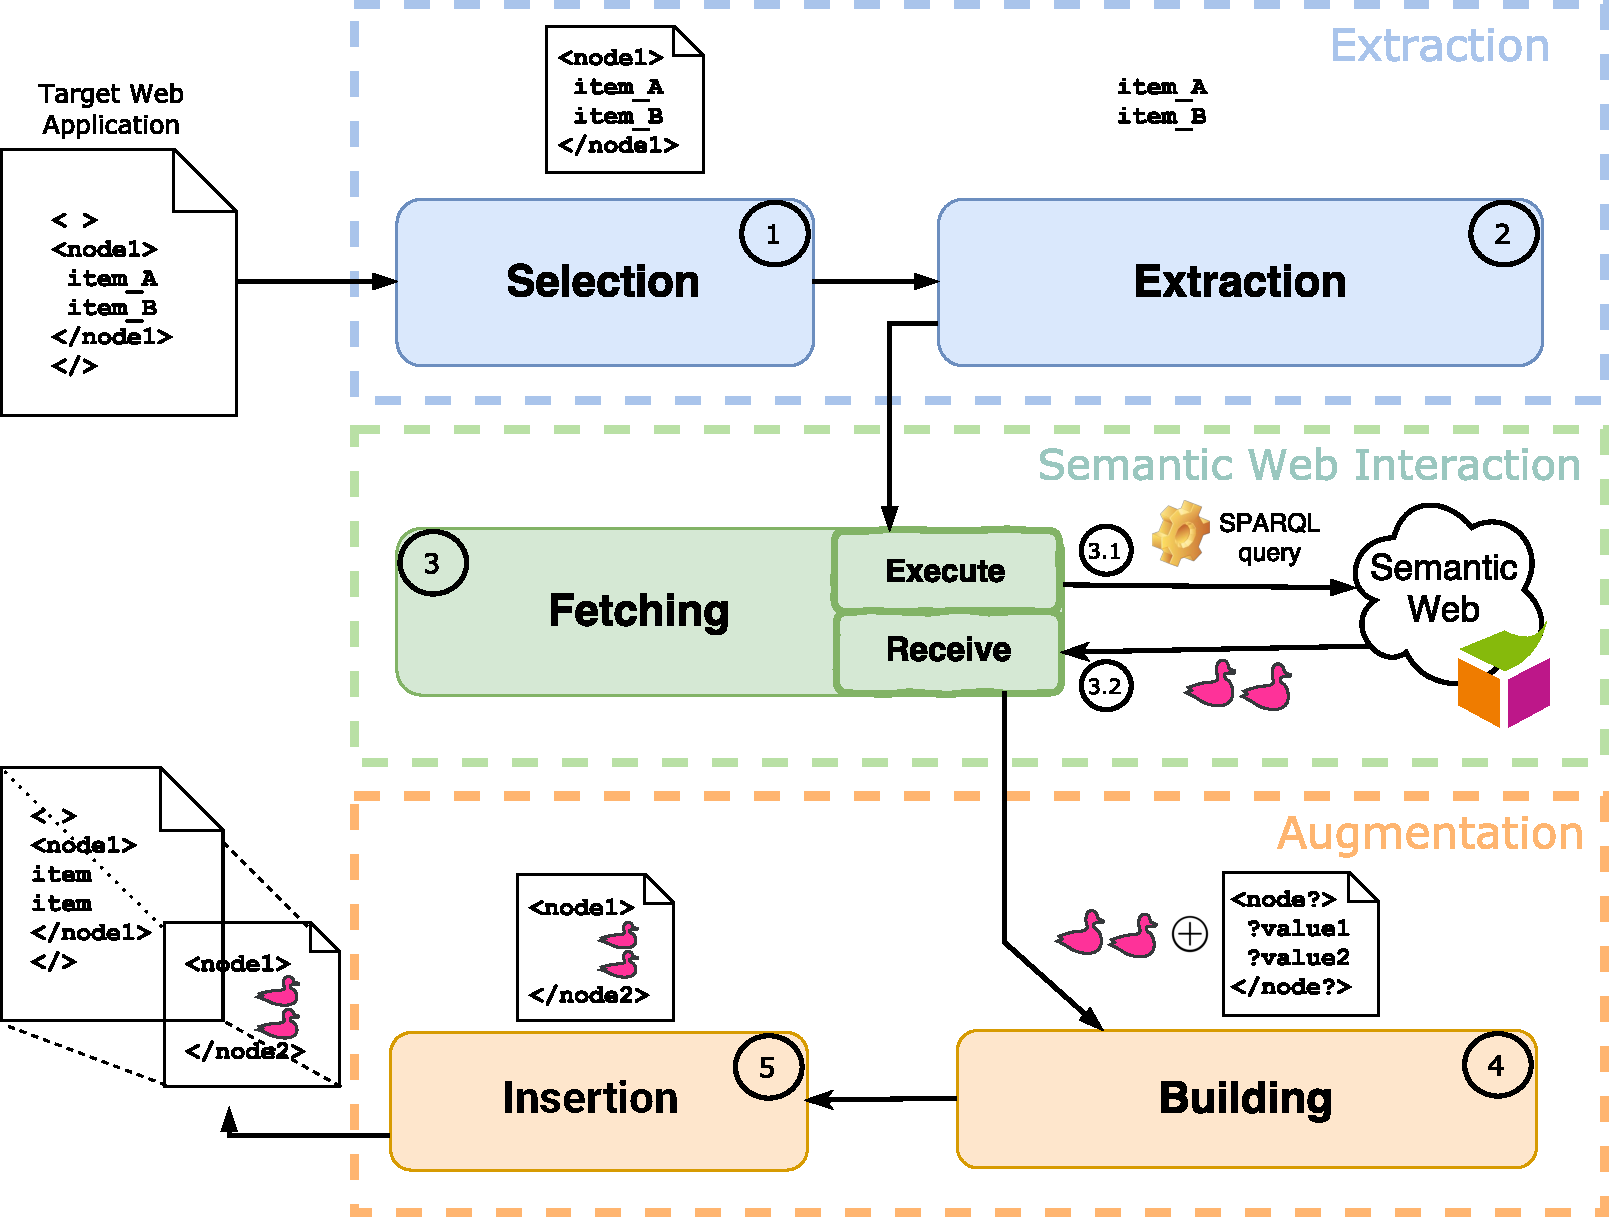
\includegraphics[width=0.80\linewidth]{SwatFmw2.pdf}
    \caption{Overview of \SWAT ~framework}
    \label{fig-framework}
\end{figure*}

This section explains the process behind the tool. Having a target Web page to be augmented, it performs three main steps. First, the extraction of information from the website. Then, it executes semantic queries against the Semantic Web (i.e., a SPARQL endpoint) to gain new information. Finally, it augments the website adding the new information. It consists of a pipeline process where each component receives, as input, the output of its predecessor.

As a guide example, we well take the IMDb\footnote{IMDb stands for Internet Movie Database. \url{http://imdb.com}} website, and say a user wants to improve the films websites by adding the amount of Oscars every cast member won. The process consists of three main steps, which we now describe.

\paragraph{Data extration} We stated that our kind of SWA will be related to the information in the current Website. In this step, these data are gathered. Following the example, these would be actor's and actress' names.

\paragraph{Data fetching} Given a generic SPARQL query and the \textit{extracted data}, this step fills the generic query with the data, producing one specific query for each one, and then run these queries against a SPARQL endpoint, obtaining the new information from the Semantic Web. In the example, the new information would be the amount of Oscars won by every cast member.

\paragraph{Building} Given an HTML template and the \textit{fetched data}, this steps generates specific HTML elements by filling the templates with the data, and inserts them in the Website, performing the Web Augmentation. In the example, the HTML element could be the amount of Oscars within a span \texttt{tag}.


\section{An End-User Development Tool for \SWAT~applications}
\label{sec-tool}

This section introduces an End-User Development Tool for building SWA, which we call SWAF-tool. It is a Web browser extension whose functionality is based upon the process described in Section \ref{sec-process}, and allows to build a Web Augmentation script based on the current Website. Web browser users are capable of enabling the tool in any Web page, initiating a wizard-like UI to configure the augmentation in a sequence of intuitive steps. The result is a script that is general enough to augment all Web pages whose DOM structure and semantics are similar to the original one. One configuration, several executions.

The primary design challenge behind this idea is the use of a pipeline process where a particular step depends on the output of the previous one plus a more specific input. Similar to a wizard application, the user configures each step sequentially: selection of the elements to be augmented, generation of the semantic query, and selection of the visual component that will contain the augmentation. Finally, the augmentation is saved to augment the desired similar Web pages. Additionally, it can be executed to test its results.

Continuing with the example described in Section \ref{sec-challenges}, a user can use the The Godfather page on IMDb\footnote{\url{https://www.imdb.com/title/tt0068646/}} to produce a script to augment this and every IMDb film page. by adding the birthdate to every person of the cast. In the following, we introduce the tool functionality using this example. Figure \ref{fig-swat_launched} shows SWAF-tool launched in the The Godfather Web page.

The tool code can be found on GitHub, at \url{https://github.com/cfsottile/swa-extension}, along with instructions on the installation and usage.
 
\begin{figure}
  \centering
    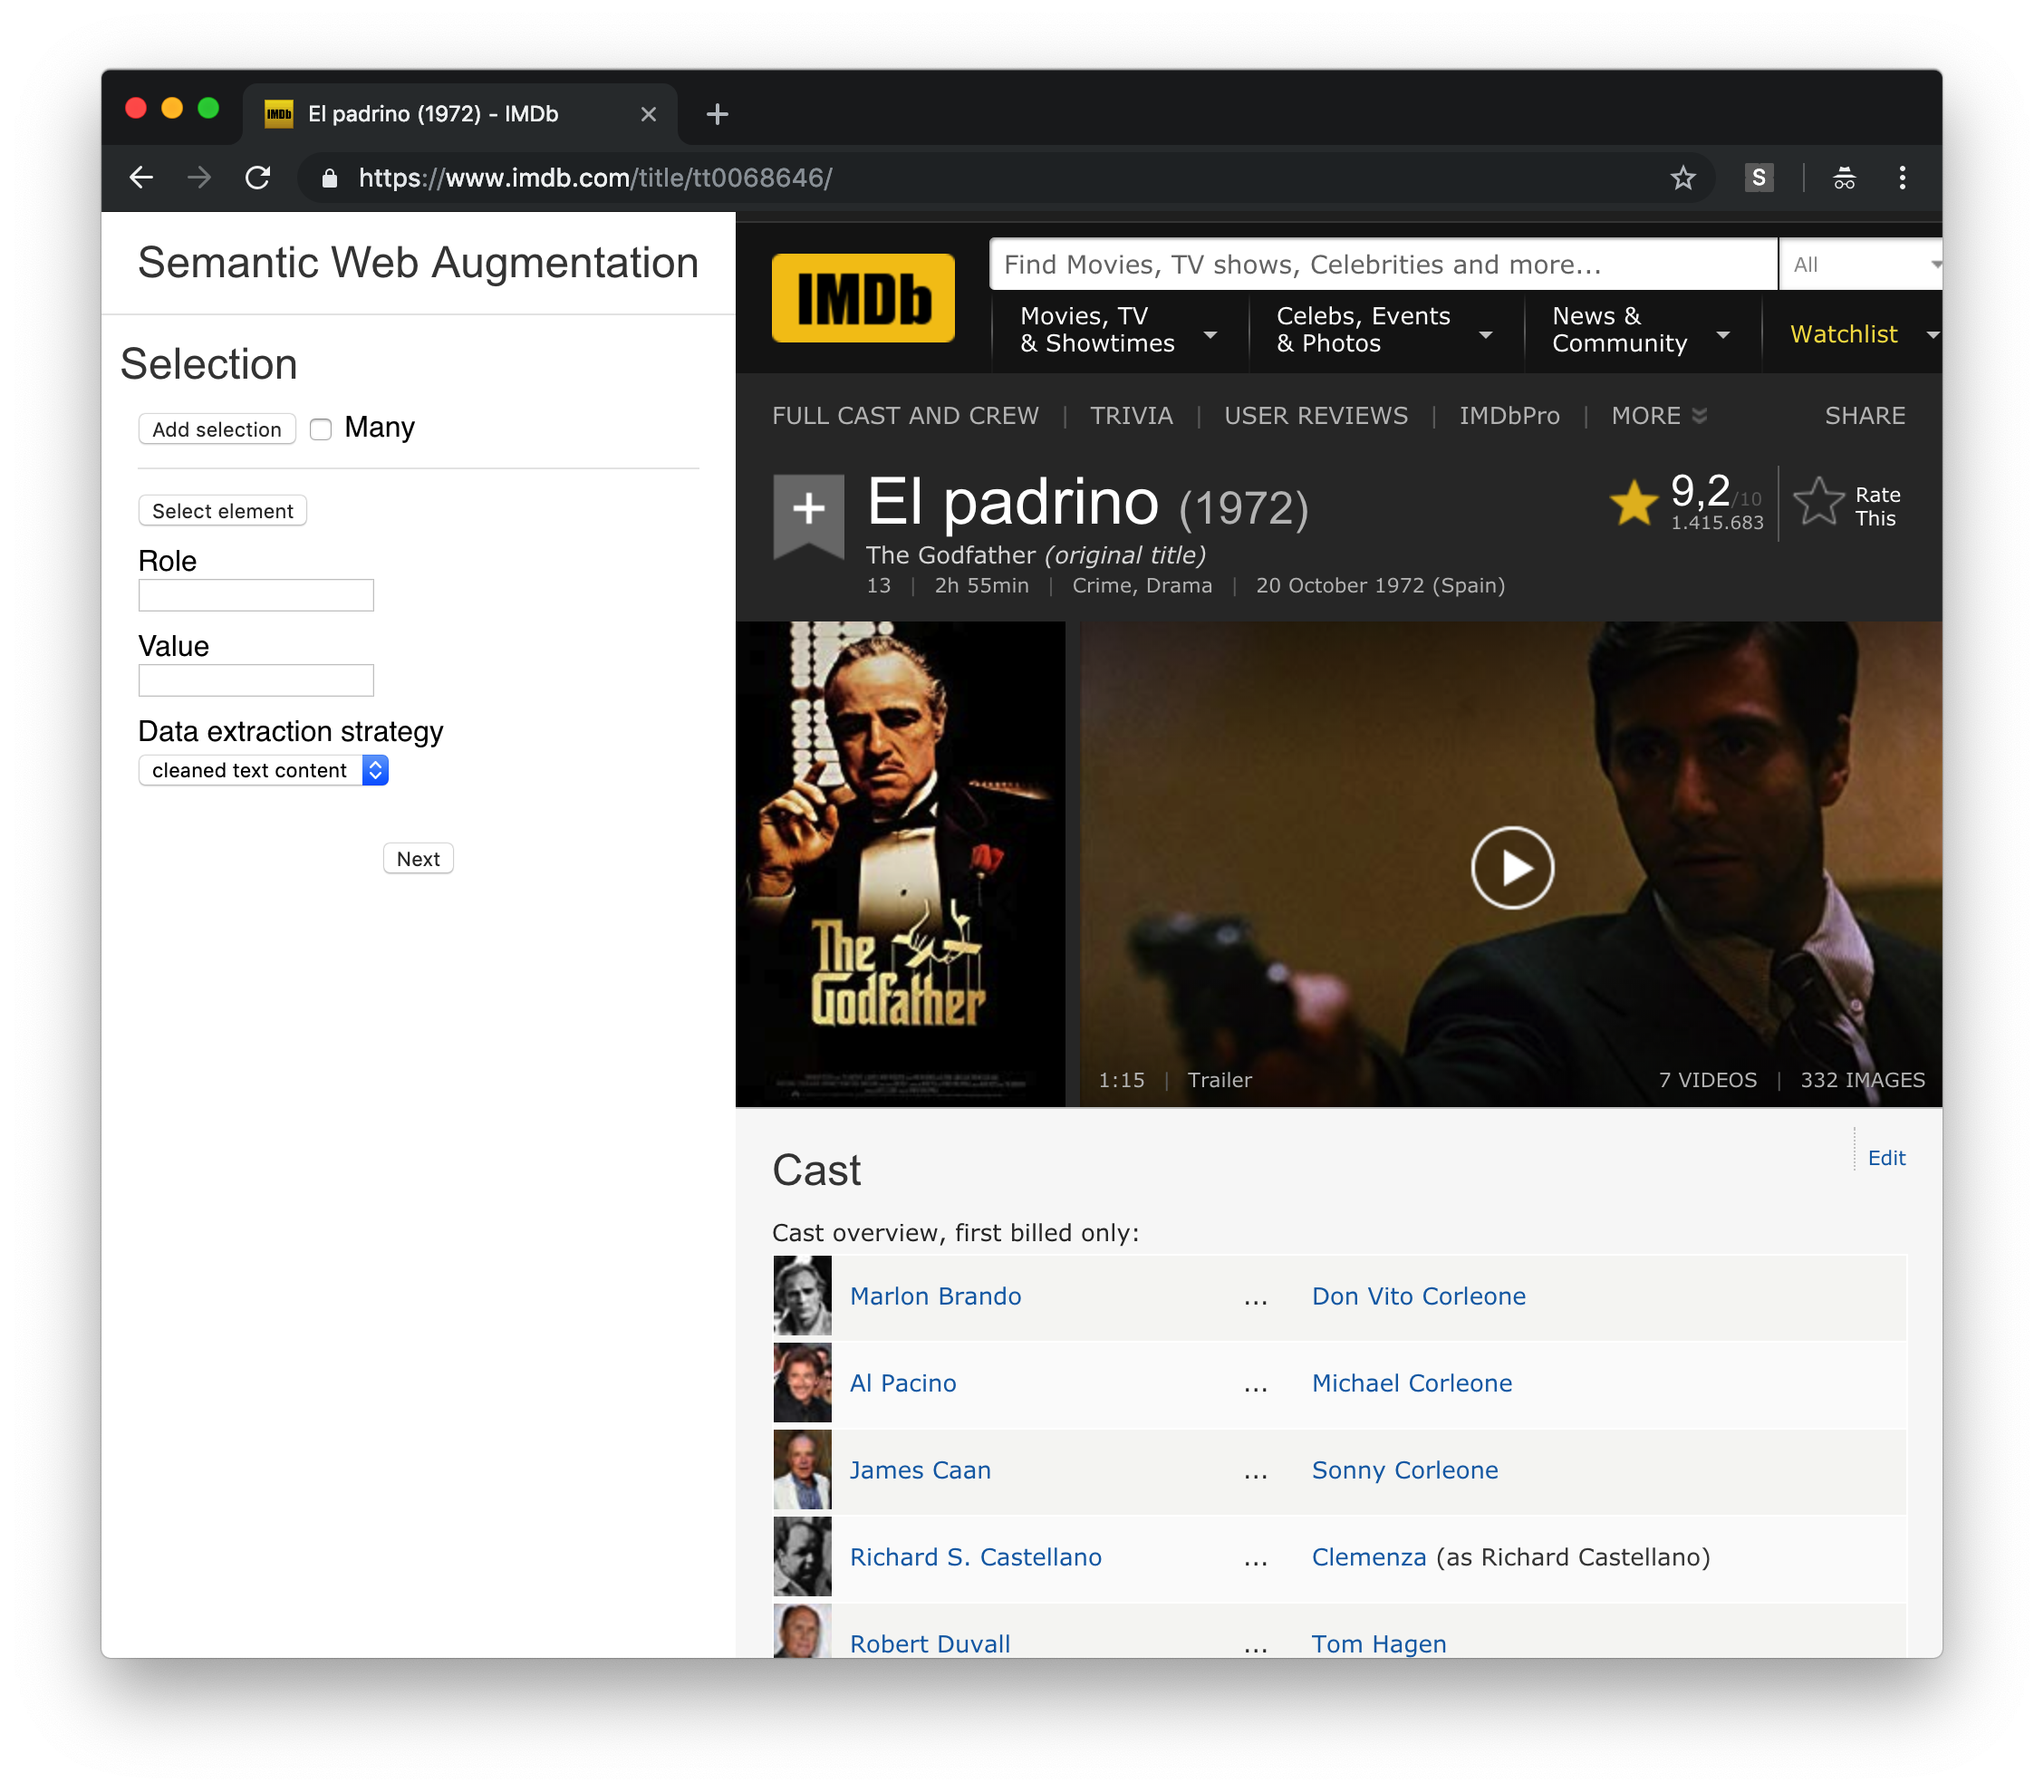
\includegraphics[width=0.99\linewidth]{tool/launched2.png}
    \caption{Tool launched}
    \label{fig-swat_launched}
\end{figure}

 \subsection{Selection and Extraction}
 \label{sec-selection}

In the first step, a user selects what DOM elements from the Web page will be used as concept label in the semantic augmentation, by enabling the selection mode and clicking them. Continuing with our example, these would be actor's names. After that, the user defines how to extract the information contained in the selected DOM element (e.g., the text content or the HREF).

Once selected the DOM element, the tool shows the \textit{value} extracted from it, and the user must specify the \emph{role}. For instance, in our IMDb's "The Godfather" example, the \emph{value} of our extracted element may be ``Marlon Brando'', and its \emph{role} would be ``actor''. The matching between value and role is required for allowing the SWAF-tool to generalize the query in terms of roles. As a consequence, the role could be replaced by a different actor or actress name and the augmentation could be reused.

Finally, if the user wants to augment more than one element, such as a list or table of similar elements (the cast of a movie falls in this category), the SWAF-tool includes a semiautomatic selection generalization, enabled by the \textit{Many} button, where the user has to select only the first and last elements of the list or table.

Additionally, if there are several concept labels, as many as needed can be added. An example could be a semantic query seeking for the population of a city, where state and country could serve to disambiguate. This query would require to take three inputs, unlike the actor's birtdate which requires only one input (the actor's name). This feature is compatible with the previously mentioned selection generalization.

Figure \ref{fig-selectionExtraction} shows this configuration step.


\begin{figure}
  \centering
    \fbox{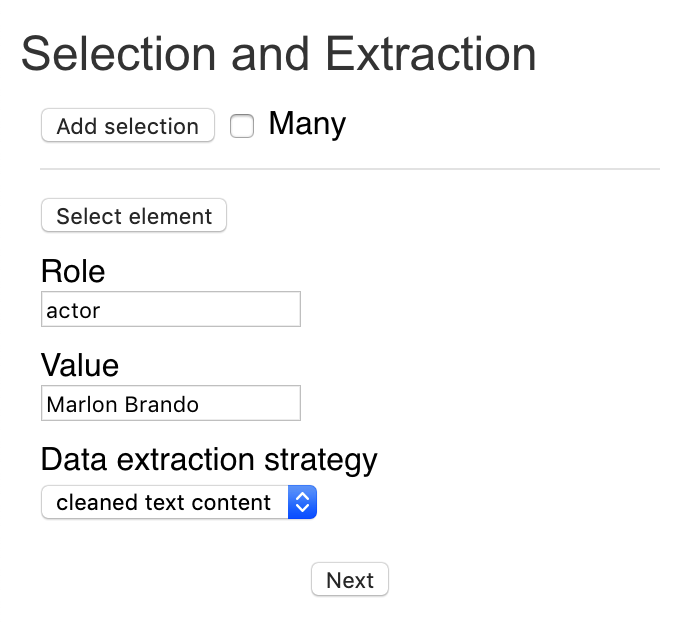
\includegraphics[width=0.80\linewidth]{tool/sel.png}}
    \caption{Selection and Extraction}
    \label{fig-selectionExtraction}
\end{figure}



\subsection{Querying}

\begin{figure}
  \centering
    \fbox{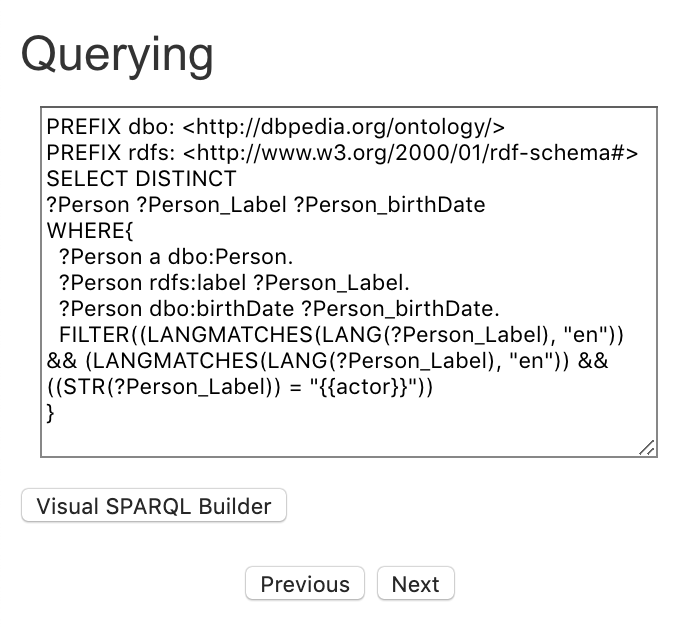
\includegraphics[width=0.80\linewidth]{tool/2_que_cut.png}}
    \caption{Querying}
    \label{fig-querying}
\end{figure}

Once the Selection and Extraction stages are done, the semantic query that will retrieve the new information from the Semantic Web must be defined. The tool provides a text input field for the query, with a link to the VSB Web application, where the user should build the query and then send it back to the input field; being the input a text field, it is flexible enough for skilled SPARQL users to build their own custom and possibly advanced queries. VSB has also been augmented adding a sidebar with elements' \emph{values} and \emph{roles}, to help users to include the values in the generated query, a generalization button, to transparently transform a specific query into a generic one, and communication buttons, to send the resulting query to the SWAF-tool input field in the target Web page. The Querying stage in SWAF-tool is shown in Figure \ref{fig-querying}, and the VSB augmentation is shown in Figure \ref{fig-vsb_augmentation}, both with the generalized actor's birthdate SPARQL query. The resulting SPARQL query will be executed in the DBpedia SPARQL endpoint, and then the query results are fetched and processed, leaving them ready to be used in the next step.

\subsection{Building}


\begin{figure}
  \centering
    \fbox{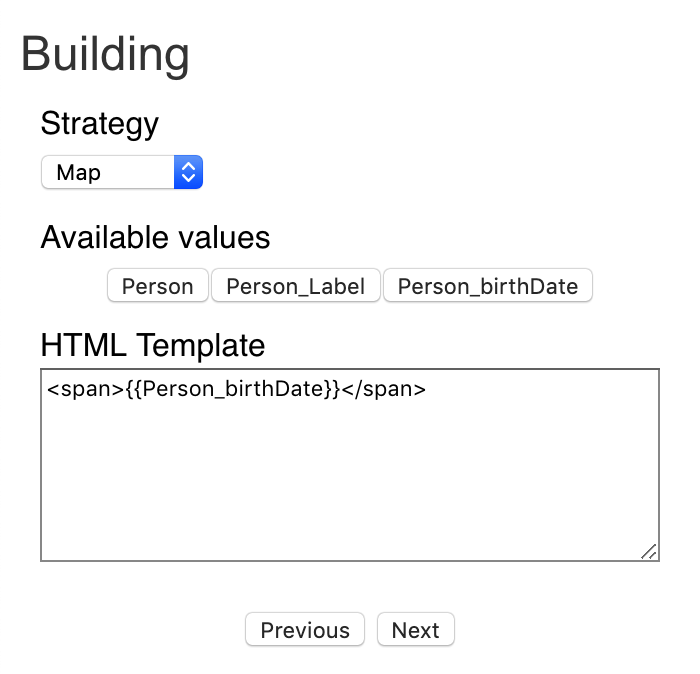
\includegraphics[width=0.80\linewidth]{tool/3_bui_cut.png}}
    \caption{Building}
    \label{fig-building}
\end{figure}


This step involves the definition of the HTML template that will be used to insert the \textit{augmentation data results} to the Web page. The user must write the HTML code including references to the augmentation data; however, the template may consist of only references, thus not being mandatory for the user to know any HTML. References to augmentation data are presented as buttons that, when clicked, are inserted into the text input for the template. The references are taken from the generic SPARQL query projection variables. Continuing with the actor's birthdate example, the template could be \texttt{\textless{}span\textgreater{}\{\{Person\_birthDate\}\}\textless{}/span\textgreater{}} as is detailed in Figure \ref{fig-building}. The tool includes different strategies in the HTML template generation, as described in Section \ref{sec-framework}: 

\begin{itemize}
\item \textbf{Map}: It maps each \textit{augmentation data result} into an HTML element. The result is a set of HTML elements to be inserted into the Web page. This will be the case of our example, where there will be one HTML element for each actor, containing his/her birthdate.  

\item \textbf{Converge}: It converges the set of \textit{augmentation data result} into a single HTML element. For instance, grouping all the birthdates together and inserting only one HTML element, which may be titled "Birthdates section", containing them.
\end{itemize}


\subsection{Insertion}

This step configures the weaving of the \textit{HTML augmentation elements} defined in the previous step. The user must choose the wanted places in the Web page to inject the augmentation elements (Figure \ref{fig-insertion}). This is done similarly to the Selection step, by selecting HTML elements from the DOM, being possible to select one or more elements according to the Building strategy.

\begin{figure}
  \centering
    \fbox{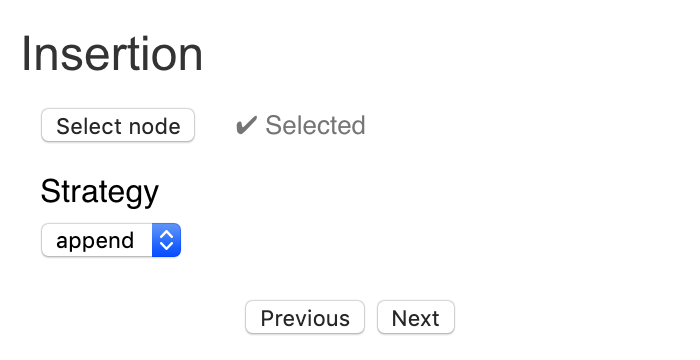
\includegraphics[width=0.80\linewidth]{tool/4_ins_cut.png}}
    \caption{Insertion}
    \label{fig-insertion}
\end{figure}


\subsection{Saving}

\begin{figure}
  \centering
    \fbox{
\includegraphics[width=0.80\linewidth]{tool/5_sav_cut.png}}
    \caption{Saving}
    \label{fig-saving}
\end{figure}


Once the previous steps are completed, the augmentation is ready to be performed. The user will then define a set of URLs where the augmentation should be applied. In our cast example, this would be \texttt{https://www.imdb.com/title/*}. The tool now shows two buttons: \textit{save}, that saves the augmentation script to apply it every time the user opens a website that match the specified expression; and \textit{try}, that performs the augmentation, letting the user see the changes that the augmentation produce in the Web page. Figure \ref{fig-finalAugmentation} shows the The Godfather page with the augmentation performed; it is of interest to note that if an actor's name is not accompanied with a date, it is because that information was not available at DBpedia.

\begin{figure}
  \centering
    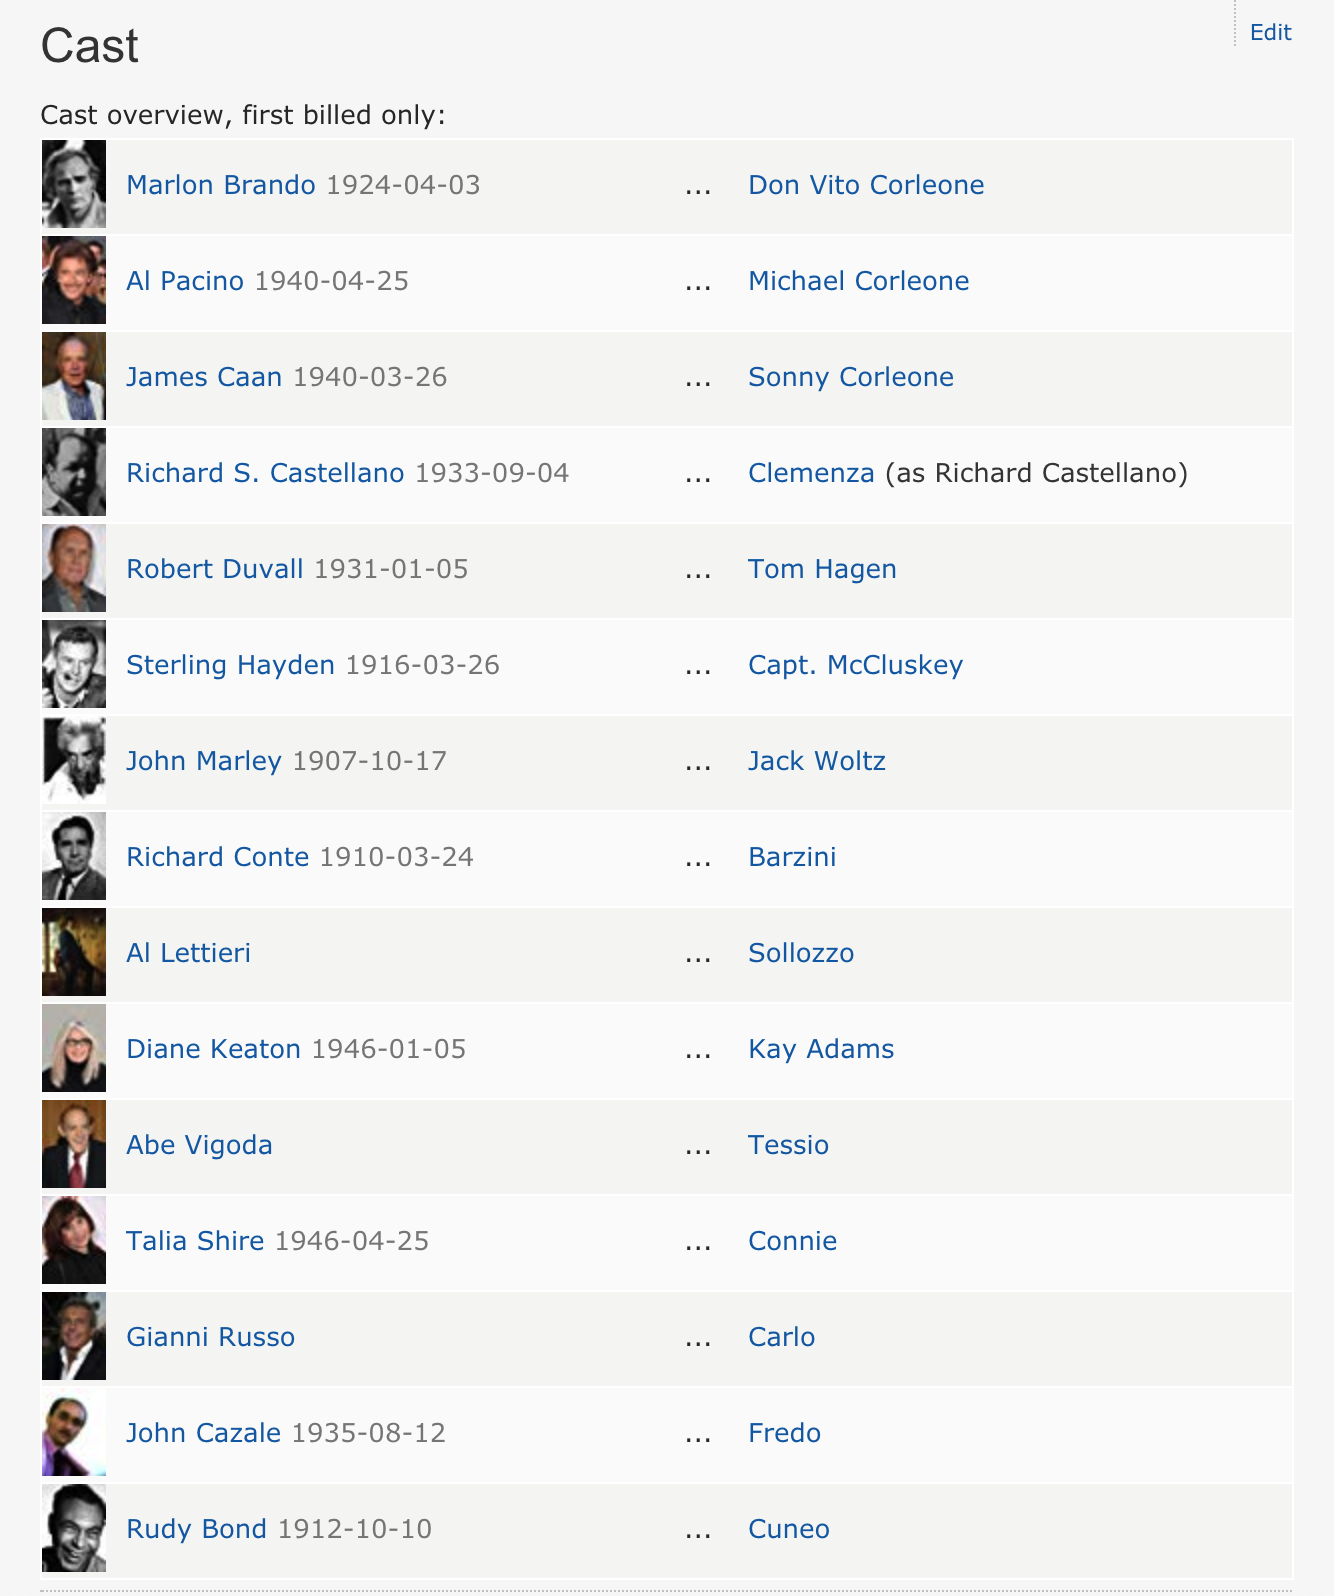
\includegraphics[width=0.85\linewidth]{tool/swa-despues.png}
    \caption{IMDb cast with the birthdate augmentation}
    \label{fig-finalAugmentation}
\end{figure}



\section{Case Studies}
\label{sec-casestudies}

This section introduces two examples of the utilization of the proposed approach to augment Web pages with the use of Semantic Web content. Both examples use DBpedia as the Semantic Web representation because it is the most important node in the LOD cloud\cite{DBpediaJournal}. 

\subsection{The Oscars augmentation for cast lists in IMDb}
\label{sec-imdb}


\begin{figure}
  \centering
    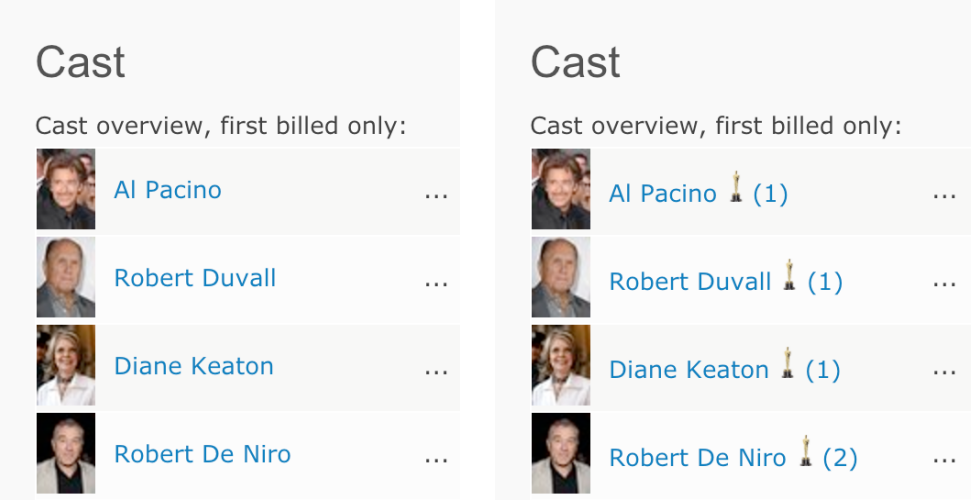
\includegraphics[width=1.0\linewidth]{oscars6.png}
    \caption{Case study: Oscars}
    \label{fig-oscars}
\end{figure}

The goal of this augmentation is to add the number of Oscars that each cast member in an IMDb page has won (not necessarily within the film). First, each actor's and actress' names are extracted from the DOM. Then, the amount of won Oscars is collected via a SPARQL query (a simplified version of this query for Al Pacino is shown in Listing \ref{l-oscars}), and the HTML template for adding the information to the website is defined (\ref{l-oscars_template}). On the left side of Figure \ref{fig-oscars} the cast list for The Godfather II is shown as appears in IMDb; on the right side, the cast list is shown after the augmentation has been executed. It has been added, besides the name of every actor, an academy award image and the number of Oscars s/he won. 


\section{Related Work}
\label{sec-related_work}
In the literature there are several references regarding the use of Semantic Web either to improve user experience, to help client-side developers to manipulate semantic data or to \textit{semantify} non-semantic pages as we discussed in the Introduction. 

The closest related works are the one introduced by Rico et al.\cite{Rico2012AData} with the concept of VPOET templates. The approach aims developers with low skills in Semantic Web technologies to create a presentation template for a specific ontology component but only for Web resources in a wiki-based framework called Fortunata; and the DBpedia Userscript project that enhances Wikipedia pages with a link to its DBpedia corresponding resource\footnote{\url{http://wiki.dbpedia.org/projects/dbpedia-userscript}}. Less related to our approach, Balloon  ~\cite{Schlegel2014BalloonWebsite} is a jQuery library to manage Semantic Web content in a Web Site. It is mainly focused on RDF browsing and visualization of RDF and ontologies data. Related to semantic augmentation, the Pundit\cite{Grassi2013Pundit:Semantics} tool provides a set of libraries to annotate content with semantic information and complement it with information generated by a SPARQL query in their context but is not feasible to be used by a third party Web application. Orabona et al.~\cite{Orabona2015AnPortals.} proposed the use of Semantic Web to enhance content management systems with the use of a triplet store. However, the use of this enhancement is developed in a server side application. 
At client-side and in the perspective of Web augmentation, Semantic Web was used with different purposes. For instance, WOA \cite{DBLP:conf/icwe/FirmenichBRWB16} presents an approach for the creation of Web augmentation layers by firstly annotating Web contents with semantic tags. In this way, the same augmentation code may be reused for any objects compliant with some specific semantic description. 
However, for the best of our knowledge, there exist no end-user programming tools for defining the weaving of information extracted from the Semantic Web in the current context of Web browsing.
 
\section{Conclusions and Further Work}
\label{sec-conclusions}

%The Semantic Web is in a mature state since many years. However, it is not common to see tools for allowing Web users communities to consume all this infrastructure. In this paper, we present a SWA framework called \SWAT, which helps \textit{userscripters} without Semantic Web knowledge to develop \textit{userscripts} oriented to Web sites contents. The Framework was instantiated for multiple examples showing the feasibility of our approach. Currently, we are designing and developing the end-User development tool, which aims to reach not only \textit{userscripters}, but also end-users with none programming skills. Future works include an evaluation with developers (for the use of the framework), and with end-users (for the tool shown in Section 5).

The Semantic Web is in a mature state since many years. However, it is not common to see tools for allowing Web users communities to consume all this infrastructure. In this paper, we present a lightweight framework for developing SWA by a client-side developer called SWAF, and an end-user development tool called SWAF-tool to create augmentation layers with SWAF. 

The approach allows end-users without any programming skills to produce generic Web Augmentation scripts that allow for enriching the contents of groups of Web pages, such as IMDb film pages. Otherwise, the augmentation task requires not only programming and knowledge management skills, but also several mining, transformation and interaction steps. The challenge of bringing these activities closer to end-users was overtaken by a pipeline process where each stage has a concise objective and predefined behaviours to accomplish it, leading the user to a straightforward non-technical experience. The case studies that we showed stand for the feasibility of our approach.



The first future work is the need for an exhaustive evaluation. The prominent prototype demonstrated well behavior, and easy to use augmentation tasks in laboratory tests. Nonetheless, we are designing usability tests with a group of developers. Additionally, more extraction and insertion strategies are in development, as well as user experience improvements. The current version of the SWAF-tool works with VSB, but there are several SPARQL query builders that could be adapted for SWAF-tool.


%
% ---- Bibliography ----
%
% BibTeX users should specify bibliography style 'splncs04'.
% References will then be sorted and formatted in the correct style.
%
% \bibliographystyle{splncs04}
% \bibliography{mybibliography}
%
\bibliographystyle{splncs04}
\bibliography{biblio}
\end{document}
